\documentclass[12pt]{report}

\usepackage[utf8]{inputenc}
\usepackage[T1]{fontenc}
\usepackage[british]{babel}

\usepackage{biblatex}
\bibliography{PIP_report}
\usepackage{amsmath}
\usepackage{graphicx}
\usepackage{verbatim}
\usepackage{subfigure}
\usepackage{hyperref}
\usepackage{csvsimple}
\usepackage[noend]{algpseudocode}
\usepackage{algorithm}
\usepackage[english=british]{csquotes}
\usepackage{pgfplots}

%\DeclareUnicodeCharacter{003A}{:}

%TODO :
% Talk about PNMC and Petri networks in the intro (variables=places, links=transitions)
% Try to graph evolution of computing time versus the number of states/nodes in a SDD
% Change the intro to talk about the matrix algorithm too, and not just Force
% Fix the bibliography (the name of a Paper should be clickable)
% Explain why Order_pre_post and Order_edges would improve
% Present the results of the benchmark with stats
% Try to graph the evolution of Span with Force, and find an otpimal criteria to end the algo.
% find another name for the "matrix" algorithm.. maybe "genetic" ?

\title{A heuristic for variable ordering in Hierarchical Set Decision Diagrams}
\author{ AZAIS Lucas \and PINON Olivier}
\date{22 Avril 2014} 

\begin{document}

\maketitle

\tableofcontents
\newpage

\section*{Introduction} %TODO : PUT IT WITHOUT THE NUMBERS !!!

Model checking consists in testing a particular model of a given system, comprehensively and automatically in order to verify if it meets a given specification. This can be achieved by generating all the possible states of a system, known as the state space. This kind of testing is especially interesting in aeronautics as it allows engineers to find all the possible flaws of a system. This method is best implemented using Computer Science as model checking involves simple but numerous operations.
\\\\
However, when the system increases in complexity, because of the combinatorial explosion, the quantity of data to deal with can reach overwhelming amounts. This is why alternative methods have been developed, and the one we have been working on is the Hierarchical Set Decisions Diagram (SDD), which consists in reducing the size of the representation of the state space by using symetries, patterns, by merging the parts that lead to the same results and summarizing it in a graph called SDD. We have based our work on Pr. Hamez’s C++ Model-Checking library called \enquote{\textit{pnmc}} \cite{pnmc}. The idea was to find a pre-processing algorithm that would speed up the computing done by \enquote{\textit{pnmc}}. An extremely efficient way to improve this computing is to find a better order for the variables used by the model checker, as it can reduce its computing time by orders of magnitude. The aim here is to design an algorithm that will find the optimal variable order, thus leading to the fastest computing time possible.
\\\\
We will first introduce the main notions required to understand how a model checker and decision diagrams work. We then started our work by trying to adapt and implement an algorithm called Force, which was originally designed for Binary Decision Diagrams where variables can only be 1 or 0. Third, we laid the basis of a brand new algorithm, based on much simpler matrices. We then ran tests to verify that the model checker was faster with a pre-processing algorithm than without, and we will present the results of these tests. Finally, several parameters influencing the quality of the order have been identified and will be presented.

\chapter{Model Checking and Decision Diagrams}

Various notions are required before even trying to explain the different techniques used to reduce computing time in a model checker.

First and foremost, a system, be it a plane, a program or a spaceship, can be represented by a set of variables which can have a variety of values (finite or not). Take one of these variables and freeze its value. Choose another variable and compute the different values it can assume, knowing the value of the first one. If this is done for each possible value of every single variable of the system, a graph can be drawn and each path in the graph (a line from top to bottom) represents one possible state of the system. This graph is then called a Decision Diagram. Its type (Hierarchical, Binary, etc) depends on the type of variables used.

\begin{figure}[!h]
  \centering
  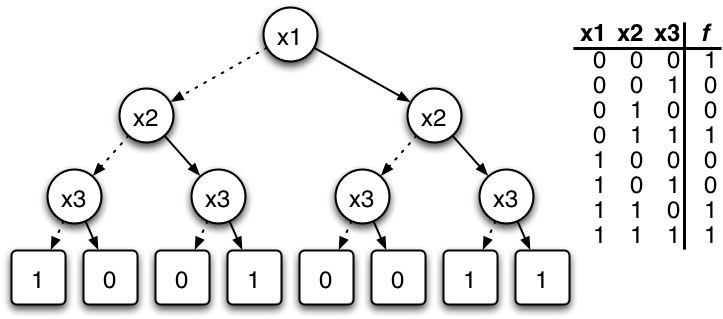
\includegraphics[scale=0.4]{images/basic_bdd.jpg}
  \caption{A simple BDD}
  \label{basic_bdd}
\end{figure}

Figure~\ref{basic_bdd} shows the comprehensive Binary Decision Diagram (BDD) of the function :
\[f(x_1,x_2,x_3) = \bar{x_1}\bar{x_2}\bar{x_3} + x_1x_2 + x_2x_3\]

However, this BDD can easily be reduced by noticing that if both $x_1$ and $x_2$ equal 1, then $f(x_1, x_2, x_3)$ will equal 1 as well, no matter what value $x_3$ assumes. If the path leading to the same value of f (0 or 1) are also joined together, the same BDD will appear as follows :

\begin{figure}[!h]
  \centering
  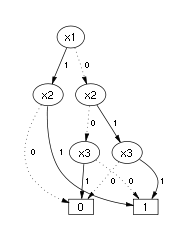
\includegraphics[scale=0.8]{images/compact_bdd.jpg}
  \caption{The same but reduced BDD}
  \label{compact_bdd}
\end{figure}

What can be noticed in this diagram is that if the variable order is changed by switching $x_3$ and $x_1$, the size of the representation will increase greatly since it will not be possible to keep track of the simplifications made above in figure~\ref{compact_bdd}. This phenomena can be highlighted in a second example, figure~\ref{reduction_bdd} where a rearrangement of the variables can lead to a much simpler BDD.

\begin{figure}[!h]
  \centering
  \subfigure{
    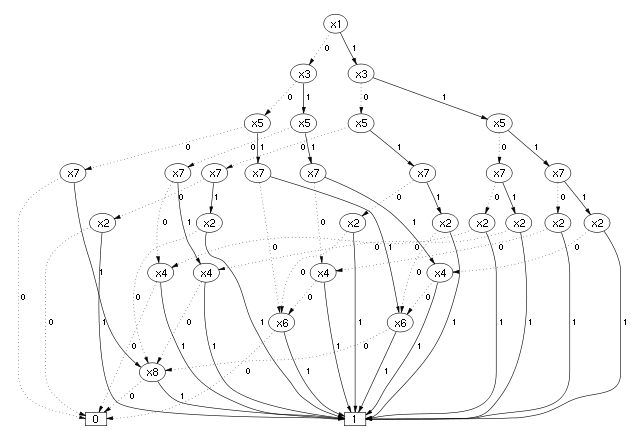
\includegraphics[scale=0.45]{images/big_bdd.jpg}
  }
  \subfigure{
    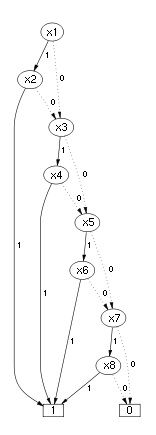
\includegraphics[scale=0.5]{images/small_bdd.jpg}
  }
  \caption{The same BDDs with different variable orders}
  \label{reduction_bdd}
\end{figure}

It is therefore readily understandable that a model checker would spend less time checking the rearranged diagram on the right, compared to the one on the left. It would thus be faster and prove less prone to mistakes. The diagram used in our algorithm, the Hierarchical Set Decision Diagram (SDD), is slightly more complex as it allows links between variables to be SDDs themselves. However, the principle remains the same and if a method is found to order BDDs, is can be adapted to SDDs.

In the case of small diagrams, a human can reorder it and let the computer handle the rest of the computation. However, for common systems, the number of variables can easily reach a thousand or more. It is then impossible for a person to even represent the diagram, making it that much more difficult to reduce its size; considering that the state space of a system has no link whatsoever with the state space of another system, the automatic modification of the variable order seems impossible. In our search to find one such algorithm, or one that would improve the computing time in most cases, an algorithm called Force caught our attention.

\chapter{Force : A powerful algorithm that can easily be enhanced}

\section{The basic version}

Taking root in the natural laws of gravity, the Force algorithm is described in \textit{FORCE : A Fast and Easy-To-Implement Variable-Ordering Heuristic} [3]. The algorithm itself is as simple as to use forces of attraction between variables. The variables are ordered on a line, given a position, and are attracted to the variables they are linked to thanks to these attraction forces. The diagram will thus organize itself in a simpler way, and should be easier to deal with afterwards.

First, the variables are defined, followed by the hyperedges which represent the links between variables. The particularity of a hyperedge is that it can bind together more than 2 variables. At the beginning, the variables are given an initial position on a line, representing the initial order. This initial order is given by the model which needs to be checked: a Petri network is parsed linearily, and the variables are given the position in which they have been parsed. After that, iterations are repeated until a suitable order is reached:

\begin{itemize}
  \item $COG$ : mean value of the variables' positions the edge connects to.
  \item variable's new $position$ : mean value of the $COG$s of its connected edges.
  \item $span$ : difference between the positions of the first and the last variables of an edge (the ones that are the most apart from each other).
\end{itemize}

\begin{algorithm}[!h]
\begin{algorithmic}[1]
\Function {FORCE}{$variables$, $edges$}
  \Repeat
    \ForAll {$edges$}
      \State {compute its $COG$}
    \EndFor
    \ForAll {$variables$}
      \State {compute its new $position$}
    \EndFor
    \State {reorder the variables according to their position}
  \Until {the total $span$ stops decreasing}
\EndFunction
\end{algorithmic}
\end{algorithm}

\begin{figure}[!h]
  \centering
  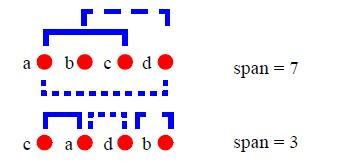
\includegraphics[scale=0.7]{images/force_span.jpg}
  \caption{A BDD before and after being reordered}
  \label{force_span}
\end{figure}

To determine the quality of an order and know when to stop, the algorithm computes the span of the order (figure~\ref{force_span}). It is the sum of the span of every hyperedge. Once the \enquote{length} of the order has settled, the algorithm is complete and gives the final order.

In figure~\ref{force_span}, 4 variables linked by 3 hyperedges can be seen. In the first order, the hyperedges are long, and once reordered, they are shorter, meaning they have a lower span. The algorithm will not be able to find a better order, it will stop and give the optimal order.

\begin{figure}[!h]
  \centering
  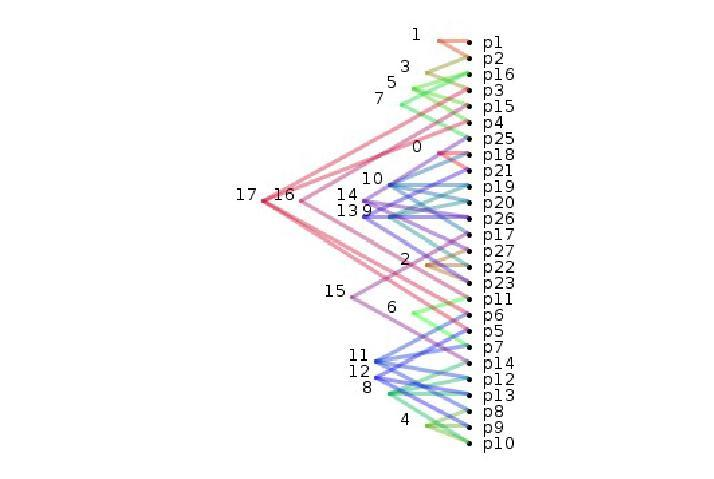
\includegraphics[scale=0.5]{images/representation_order.jpg}
  \caption{A graphic representation of the SDD}
  \label{order_graph}
\end{figure}

To help us in our work, we created a program to display the variable order. It particularly helps with finding symetries in a graph, or patterns that should be studied further. Figure~\ref{order_graph} shows a graphic output of that program, and represents an SDD.

On the left are the hyperedges that connect the different variables. The further they appear on the left, the higher their span. On the right are the variables (known as places in this case, hence p1, p2, etc)

\section{Force's execution time and termination criteria}

\begin{figure}[H]
  %\centering
  \begin{center}
  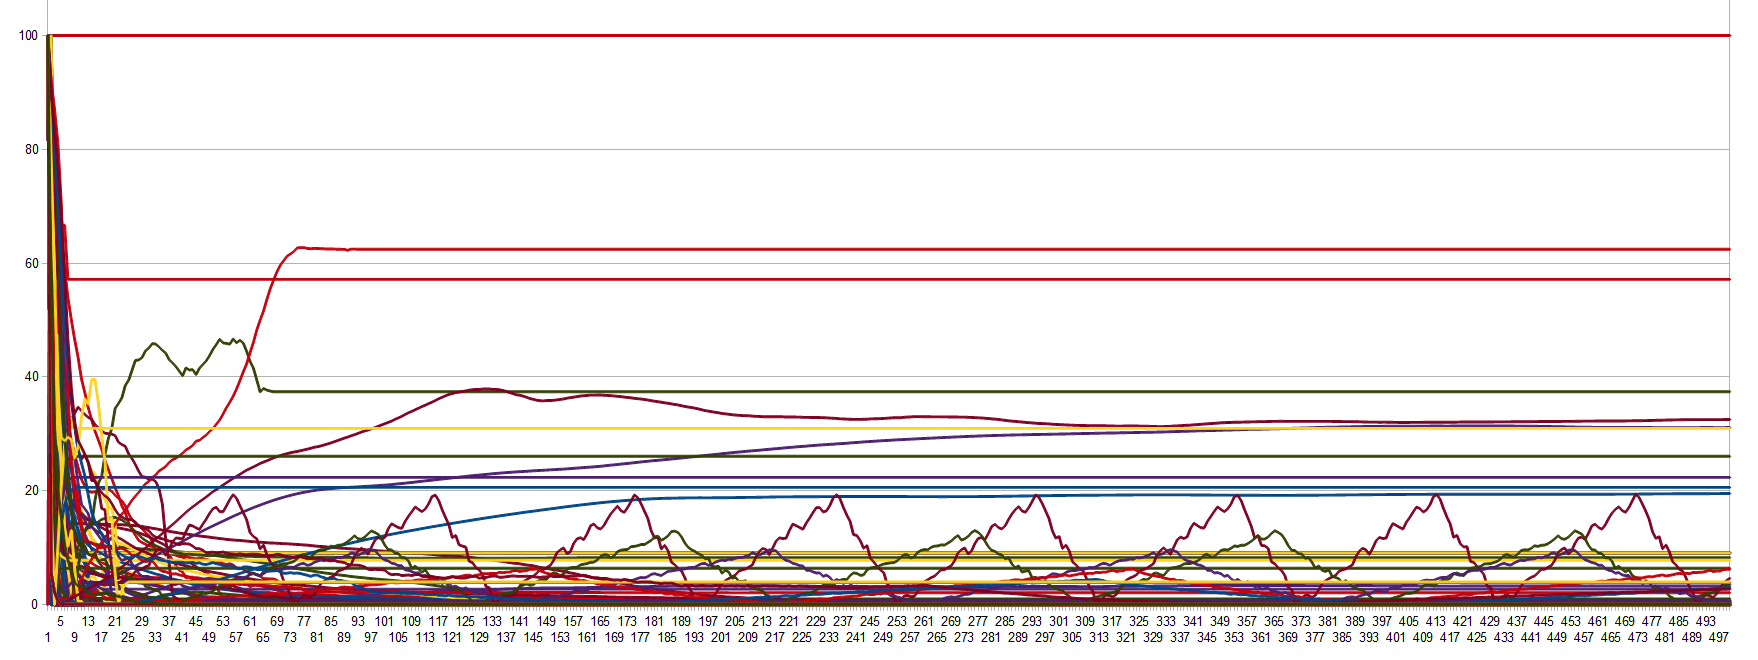
\includegraphics[width=1\textwidth]{images/force_plot.png}
  \end{center}
  \caption{The evolution of the span during Force, for a pool of 162 examples. In absciss are the number of iterations. The ordinates start at 0\% with the minimal span encountered during the evolution, and end at 100\% with the maximal span.}
  \label{force_plot}
\end{figure}

Figure~\ref{force_plot} shows the evolution of the $span$ during Force's execution. In most of the 162 cases the span reaches its minimal value within the first ten iterations, but there are a dozen cases that behave in another way: they first reach a minimal value, but then the span increases to finally stabilize at a higher value. There is also cases where the span settles in a periodic evolution. Considering those two cases, stopping Force as soon as the span stops decreasing might seem like the best idea, but there is one last case: the span might increase for a while, but then decrease to reach a final, much lower, value.
The solution we finally chose was to terminate Force when the span had stayed higher than its minimal value for 100 iterations and establish the final order as the one corresponding to the minimal span reached during these iterations.

\begin{figure}[H]
    \subfigure[duration vs the number of variables]{
      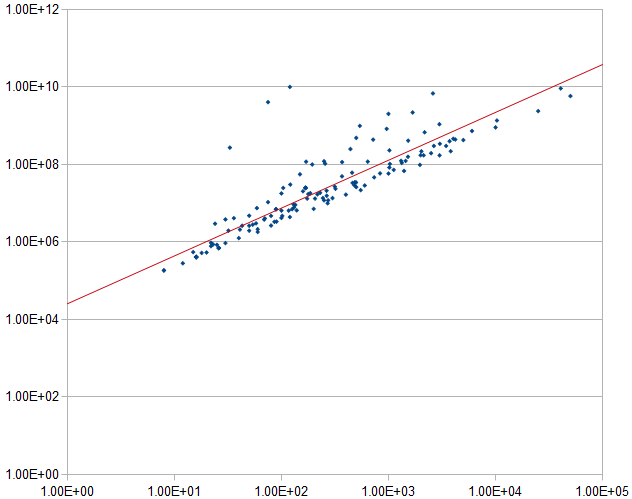
\includegraphics[width=0.45\textwidth]{images/time_vs_var.png}
      \label{time_vs_var}
    }
    \subfigure[duration vs the number of edges]{
      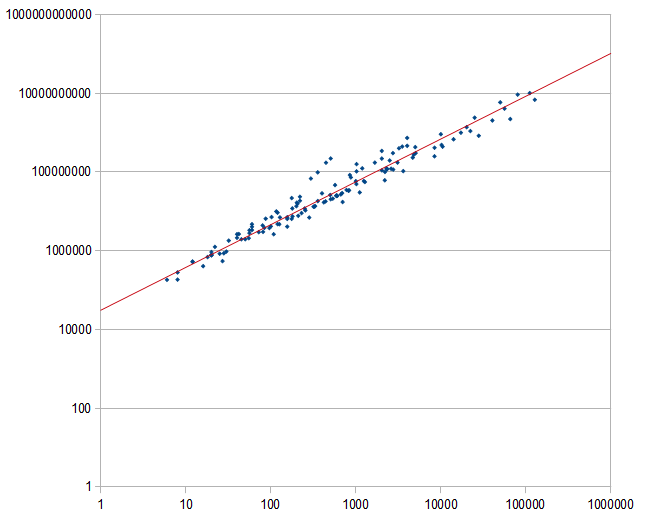
\includegraphics[width=0.45\textwidth]{images/time_vs_edges.png}
      \label{time_vs_edges}
    }
    \subfigure[duration vs the sum of the numbers of variables and edges]{
      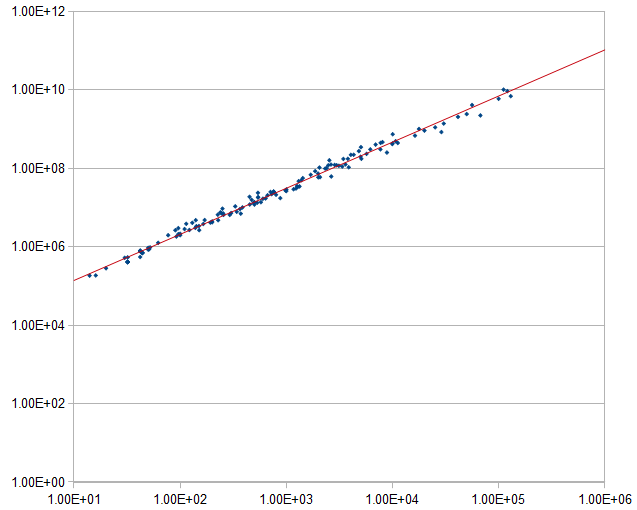
\includegraphics[width=0.45\textwidth]{images/time_vs_(var+edges).png}
      \label{time_vs_(var+edges)}
    }
    \subfigure[duration vs the product of the numbers of variables and edges]{
      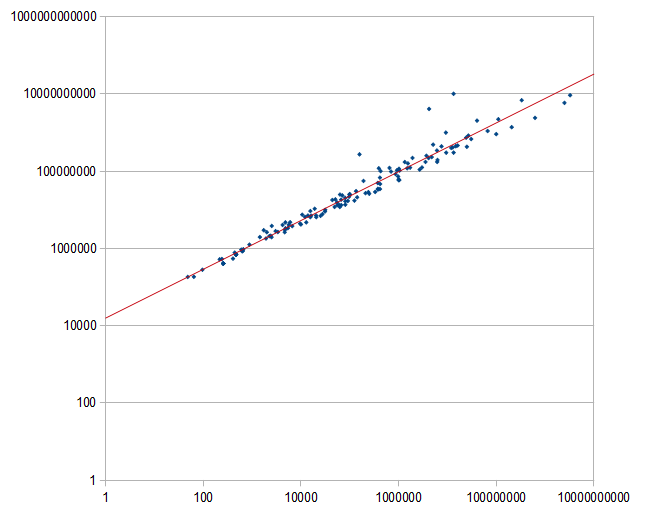
\includegraphics[width=0.45\textwidth]{images/time_vs_(var_x_edges).png}
      \label{time_vs_(var_x_edges)}
    }
\label{force_duration}
\caption{Duration of Force's execution (in ns) versus the samples' complexity, in a logarithmic scale.}
\end{figure}

The data that fits best its regression is ~\ref{time_vs_(var+edges)} with a correlation coefficient of R=0.993 and the model is $time({\mu}s)= {9.2}*x^{1.17}$. For example with one of the largest model that has $5*10^4$ variables and $5*10^4$ edges, the duration of Force is $6.1$ seconds and the equation gives an estimation of $6.5$s.

\section{The PRE-POST enhancement}

Because the model-checker we use is based on Petri networks, there is another information we can use to build the order. As a matter of fact, the links (also called \enquote{transitions}) represent operations used on the variables to build the graph, and therefore have a direction. It means that a variable depends on another, and the link between variables can be unidirectional or bidirectional. It seems intuitive to put a variable after the ones it depends on. A variable others depend on is called PRE, a variable depending on another is a POST, and a bidirectional link involves PRE-POST variables. Using that information before each iteration of the algorithm proved to help decrease the span further in some cases.
This operation can be done as follows :
%TODO explain why this can enhance the computation

\begin{algorithm}
\begin{algorithmic}[1]
\Function {Order PRE-POST}{$variables$, $edges$}
  \State {compute the edges' COGs}
  \State {sort the $edges$ to have the ones with the highest span at the beginning} %TODO: this is actually order_pre_post reversed
  \ForAll{$edges$}
    \State {sort the $variables$ in order to have the $PRE$, then the $PRE-POST$ and finally the $POST$}
    \State {place these $variables$ in that order around the edge's $COG$}
  \EndFor
  \State {compute the new order according to the $variables$' positions}
\EndFunction
\end{algorithmic}
\end{algorithm}

In theory, sorting the edges at the beginning allows the order not to be changed too much, while still forcing the transition types to be as sorted as possible. Hence when processing an edge, we take the variables from all over and gather them at the edge's COG. Right after being processed, the edge has a minimal span; but because processing the next edges will also move the variables, it will progressively be unmade. This is the reason why we start by applying it to the edges with the highest span, and end with those with the lowest. The edges we process first probably won't respect the rule because the future operations will unmake the first ones; however we want to make sure that the edges with the smallest span do respect it, and because they are processed last, they will end with a minimal span.

\section{Sorting the edges}

The last enhancement we tried was to order the edges according to their number of variables :

\begin{algorithm}
\begin{algorithmic}[1]
\Function {Order Edges}{$variables$, $edges$}
  \State {do a stable sort of the $edges$ according to the number of variables they connect to}
  \State {compute the $edges$' $COG$s according to that order}
  \State {compute the variables' new positions according to the $edges$' $COG$s}
\EndFunction
\end{algorithmic}
\end{algorithm}

This operation may reduce the model-checker's computing time because when operations are applied on a SDD to construct it, these operations propagate from the top of the diagram and then are repeated further in the diagram until they reach a certain criteria. ??????????????

\chapter{A genetic algorithm}

Seeing what could be achieved with relatively simple methods, we designed another algorithm based on matrices, the most widely used representation for problems in mathematics. The rationale was to speed up the calculations by simplifying the representation of the Hyper Edges.
\\\\
The principle is that a matrix will represent one model. The lines represent the variables of the model, thus the current variable order, and the columns represent the different operations (as know as the hyper edges) used to build the state space. If a variable is involved in a certain operation, a 1 is inserted at the intersection of the corresponding line and column. After having considered all the variables and their link to the hyper edges, the rest of the matrix is filled with zeros (\ref{example_matrix}).

\begin{figure}[!h]
  \centering
  $\bordermatrix{
  ~ & h_1 & h_2 & h_3 & h_4 & h_5 & h_6 \cr
  v_1 & 1 & 1 & 0 & 0 & 1 & 0 \cr
  v_2 & 0 & 1 & 1 & 0 & 1 & 0 \cr
  v_3 & 0 & 1 & 0 & 1 & 0 & 1 \cr
  v_4 & 1 & 0 & 0 & 1 & 0 & 0 \cr
  v_5 & 0 & 1 & 0 & 1 & 1 & 1 \cr
  v_6 & 1 & 0 & 1 & 0 & 0 & 0\cr
  }$
  \caption{A binary matrix representing a random model}
  \label{example_matrix}
\end{figure}

As opposed to Force, this representation of a model requires a new way to determine the end of the algorithm. As a matter of fact, the span cannot be computed the same way as before. In the following paragraphs, the term \enquote{\it{norm}} will be used to designate the value representing whether an order will be considered \enquote{good} or not. It is the equivalent of the span. 
This norm can be computed as follows:
For each column, the number of $0$ between the first and last $1$ of that column is determined. After that, the results from each column are added together, and give the norm of the matrix. It can be seen as the \enquote{area} of the matrix. The lower the area, the more separated the variables will be, and just as it was intuited for Force, the longer the model checking should be.

Like before, the only available action on the model is to change the variable order and this is done here by switching two lines together. Several versions of the algorithm were tested, trying various techniques to reduce the norm, unfortunately none has proven significantly useful so far. 

We started by trying to find a way, given a random binary matrix, to get the ones closer from each other. The following pseudo-code has been tried :

\begin{algorithm}
\begin{algorithmic}[1]
\Function {matrix\_order}{$matrix$}
  \While {the norm keeps decreasing}
    \State {$c_1$ = the column with the highest norm}
    \State {switch the rows of the first 0 after the first 1 and the last 1 of the column}
    \If {$newNorm \geq oldNorm$}
      \State {try again with $c_2$ : the column that has the second highest norm}
    \EndIf
  \EndWhile
\EndFunction
\end{algorithmic}
\end{algorithm}

Although this algorithm works satisfactorily for small matrices, complex models contain thousands of variables, and a switch that lowers the norm of a single column will most certainly increase the norm of a hundred others.
After several attempts at finding an algorithm that worked in every case, it became increasingly clear that finding one such algorithm would not be easy, and may not even be possible.

Therefore, we decided another approach, that could be easily implemented and which would certainly yield acceptable results : a genetic algorithm. 

The algorithm consists in 3 distinct phases :

\begin{itemize}
  \item Initialization : a set of matrices is created from the original matrix, which are created by switching 2 rows at random.
  \item Mutation : from each matrix in the aforementioned set, a certain amount of matrices is created once again, thus creating a pool of matrices.
  \item Selection : this pool is then sorted from the lowest to the greatest norm, and a few of the best matrices are selected to act as the set for the next mutation.
\end{itemize}

The last two phases are repeated until the end. And what is particularly interesting with this algorithm is that the longer it is run, the better the results. This way, the algorithm can be adjusted according to the time available and the expected results. The algorithm will stop after all the iterations have been completed.
After the end, the best matrix in the pool is selected, and by tracing back the different rows switched, the new order is created.

In order to choose the amount of matrices to create, 4 variables must be given to the algorithm :

\begin{itemize}
  \item $INITIAL\_POPULATION$ : the initial number of matrices created from the original one.
  \item $ITERATION\_NUMBER$ : the number of iterations of the algorithm. This is the primary way to improve the order and have a lower norm.
  \item $MUTATION\_SIZE$ : the number of matrices created by the mutation process. Every matrix of the current matrix set will create that number of matrices.
  \item $SELECTION\_SIZE$ : the number of matrices selected at the end of an iteration, it will influence genetic mixing, and may better the results of the algorithm.
\end{itemize}

All these variables allow the algorithm to be extremely flexible to the needs of the user. 

\chapter{Experimental results}

\section{Force algorithm}

The Force algorithm and the enhanced version of Force have been tested using some of the most common computer science problems. In each case, we prompted the time needed to apply the model checker and get a solution.

\begin{figure}[!h]
  \begin{center}
    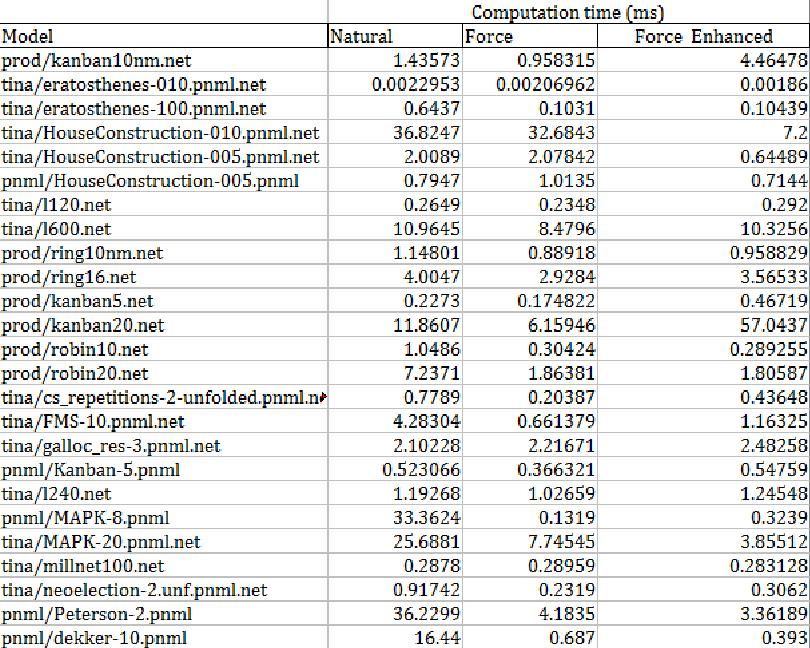
\includegraphics[scale=0.33]{images/force_results.jpg}
    \caption{Experimental results using the Force algorithm and its enhanced version}
    \label{force_results}
  \end{center}
\end{figure}

\begin{figure}[!h]
  \begin{center}
  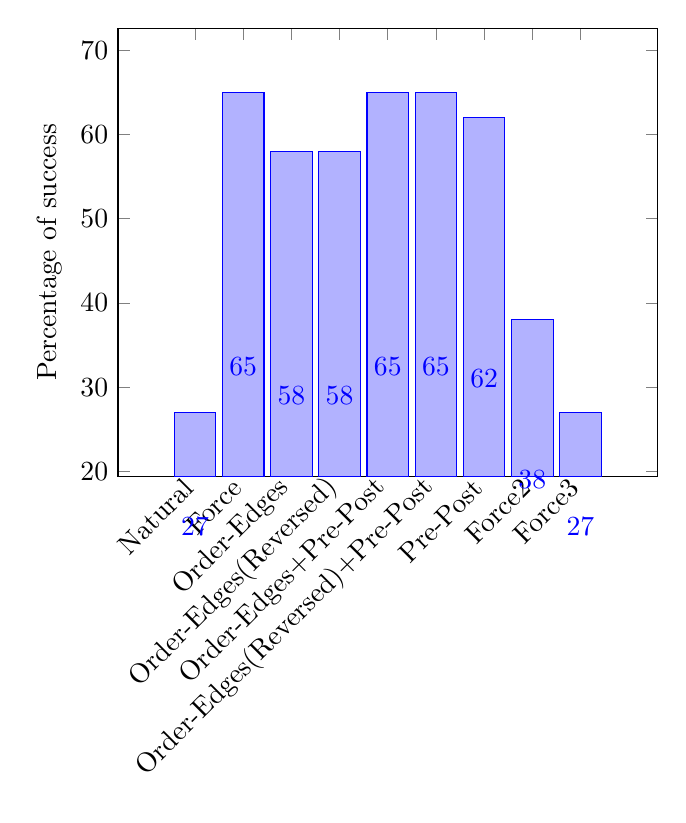
\begin{tikzpicture}
  \begin{axis}[
    ybar stacked,
    bar width=15pt,
    nodes near coords,
    enlargelimits=0.2,
    ylabel={ Percentage of success },
    symbolic x coords = {
      Natural,
      Force,
      Order-Edges,
      Order-Edges(Reversed),
      Order-Edges+Pre-Post,
      Order-Edges(Reversed)+Pre-Post,
      Pre-Post,
      Force2,
      Force3
    },
    xtick=data,
    x tick label style={rotate=45,anchor=east},
    ]
\addplot+[ybar] plot coordinates {
  (Natural,27)
  (Force,65)
  (Order-Edges,58)
  (Order-Edges(Reversed),58)
  (Order-Edges+Pre-Post,65)
  (Order-Edges(Reversed)+Pre-Post,65)
  (Pre-Post,62)
  (Force2,38)
  (Force3,27)
};
\end{axis}
\end{tikzpicture}
\end{center}
\caption {Percentage of success for each algorithm, over the cases where at least one algorithm succeeded}
\end{figure}

The tests have shown that although Force does give better results in many cases, the most significant results are achieved with the enhanced version of Force. For the House Construction 010 problem, computation has been improved fourfold, and it gives similar results in many cases. However, there are still cases where the computing time has not been improved. It appears that if the order is already considered \enquote{good}, the algorithm tends to worsen it. Further work will determine the reasons behind such behavior.

\section{Genetic algorithm}

In addition to the natural order, 6 different configurations have been tested, summarized in the following table:

\begin{table}[!h]
  \begin{center}
    \hspace*{-0.8cm}
    \scalebox{0.8}{
      \begin{tabular}{lcccccc}
        Configuration       & Short & Medium & Long & Short-iteration & Medium-iteration & Long-iteration \\
        INITIAL\_POPULATION & 40    & 40     & 40   & 40              & 40               & 40             \\
        ITERATION\_NUMBER   & 20    & 100    & 200  & 100             & 200              & 400            \\
        MUTATION\_SIZE      & 20    & 40     & 50   & 20              & 20               & 20             \\
        SELECTION\_SIZE     & 10    & 5      & 2    & 3               & 3                & 3             
      \end{tabular}
    }
    \label{genetic_configuration}
    \caption{Variables used for the different results}
  \end{center}
\end{table}

\begin{table}[!h]
  \begin{center}
    \hspace*{-0.52cm}
    \scalebox{0.6}{
      \begin{tabular}{l|c|c|c|c|c|c|c}
        \bfseries Model & \bfseries Natural & \bfseries Short & \bfseries Short iteration & \bfseries Medium & \bfseries Medium iteration & \bfseries Long & \bfseries Long iteration
        \csvreader[head to column names]{csv_files/genetic_results.csv}{}
        {\\\hline\csvcoli&\csvcolii&\csvcoliii&\csvcoliv&\csvcolv&\csvcolvi&\csvcolvii&\csvcolviii}
      \end{tabular}
    }
    \label{genetic_results}
    \caption{Experimental results using the genetic algorithm, compared to the natural order (in percentages)}
  \end{center}
\end{table}

Like Force, the genetic algorithm has been tested in the same cases, with the same computer, so that the benchmarks can be compared.

After running the benchmark, it appeared that the genetic algorithm only finishes the calculation in the cases where the natural order finishes. As the algorithm does not change the nature of the model, and does not use a particular representation like Force and the hyper-edges, it seems only logical that the percentage of success is kept at the same level.

It can be first noticed that no order of magnitude is gained nor lost due to the algorithm. The best that was achieved was cutting the computing time by half. However, there are still many cases in which the genetic algorithm worsen the order in a way that is not fully understood yet. From that fact can be deduced that just as we had to take more parameters into account for Force, the quality of the order is not entirely dependent on the norm of the matrix used to represent the model. Therefore, a future work would consist in finding the various parameters that influence the order, and implement them in a new algorithm that may yield better results.

\section{Comparison of the two algorithms}



\newpage
\section*{Conclusion}

The Hierarchical Set Decision Diagrams have been designed to be a fast and efficient representation of state spaces for model checking. Although using SDD cut the memory usage of the model checker, further work on the SDD is possible to greatly enhance its computing time. We showed that applying a pre-processing algorithm to determine an optimal variable order can sometimes greatly reduce the time needed to run the model checker. The enhanced version of Force seems to be efficient in most cases.

After more than 120 hours of benchmarking, we can confirm that Force takes very little time to be applied and seldom deteriorates the variable order. However, some cases remain where nor the initial order, nor the Force order lead to a reasonable computing time. The parameters influencing the quality of the order could not be identified, and a better understanding of these parameters would surely lead to a more efficient version of Force. Future studies should aim at determining why certain models reject the use of Force, and what could be done to improve it.

A solution might also be to try and imagine new algorithms, but since SDDs are so difficult to grasp, it will be some time before we achieve better results than Force. The genetic algorithm we designed works very well in many cases, but takes a lot more time. This is why it is crucial to have various algorithms available, in order to apply the one suited for the situation.

\printbibliography

\end{document}